\section{Related Work}
\label{sec:related}
When it comes to GNN interpretability, there are a few main methods. The first that started the field of GNN interpretability was GNN Explainer \cite{ying_gnnexplainer_2019} which also provided a suite of general benchmarks that most methods have utilized as a framework for analyzing the effectiveness of their explainer framework. Another major piece of work in the field has been the parametrized-graph explainer (PGExplainer) \cite{luo_parameterized_2020} that took GNNExplainer and parametrized it with a deep neural network for faster inference times and more robust interpretation. Along with these two, a few other more recent explainers such as SubgraphX \cite{yuan_explainability_2021} and Gem \cite{lin_generative_2021} have introduced new ideas into the field with a variety of approaches to the problem of GNN interpretability. To date, there seems to be no fully Bayesian method to the problem of GNN interpretability.

In addition to these works, the work of SERGIO \cite{dibaeinia_sergio_2020} will be introduced as it will be utilized later on to generate a new class of experiments that GNN Interpretability methods can be benchmarked against. This work provides causal graph structures that give a guaranteed groundtruth for interpretation.

\subsection{GNN Explainer}
The full version of GNNExplainer attempts to learn both a node interpretation and edge interpretation. For this work, only the edge interpretation part of the framework was utilized. GNN Explainer attempts to solve the objective outlined in \S\ref{sec:intro-interp}, by only trying to learn $\mathcal{W}_i$ while treating $\mathcal{E}_i = E$. In this framework, GNN Explainer enforces that for any $e \in E$, $W(e) \geq \mathcal{W}_i(e)$. Then to get the argmax, GNNExplainer treats $\mathcal{W}_i$ as a random variable. Then the goal get transformed to 
\begin{align*}
	\argmin_{\mathcal{W}_i} \mathbb{E}_{w \sim \mathcal{W}_i} [H(\phi(v_i, \mathcal{X}, E, w))]
\end{align*}
This still remains intractible, so GNNExplainer attempts to make this simpler by using Jensen's inequality. Note that this is not a reasonable application of Jensen's since $\phi$ as a GNN has almost no hope of being convex. Nonetheless, using Jensen's inequality gives
\begin{align*}
	\argmin_{\mathcal{W}_i} H(\phi(v_i, \mathcal{X}, E, \mathbb{E}[\mathcal{W_i}]))
\end{align*}
This is still quite intractable if $\mathcal{W_i}$ is a full joint distribution over all $e \in E$. Therefore, GNNExplainer attempts to use a mean field approximation for $\mathcal{W}_i$ where the edge interpretation is decomposed into the product of Bernoulli distributions meaning that each edge weight is an independent Bernoulli distribution with mean equal to the underlying probability of the variable. Specifically,
\begin{align*}
	\mathcal{P}(\mathcal{W}_i) = \prod_{(v_j, v_k) \in E} \mathcal{W}_i[v_j, v_k]
\end{align*}
with each $\mathcal{W}_i[v_j, v_k]$ is a value between $[0, 1]$ representing a Bernoulli variable for each edge in the underlying graph as defined by $E$. In this case, if the classification for a node is $c$, GNNExplainer performs direct gradient descent on this array of values to minimize
\begin{align*}
	\argmin_{\mathcal{W}_i = \{\mathcal{W}_i[v_j, v_k] \mid (v_j, v_k) \in E\}} -\sum_{c=1}^C \mathbb{1}_{y = c} \log \mathcal{P}(\phi(v_i, \mathcal{X}, E, \mathcal{W}_i) = c)
\end{align*}
While there is some probabilistic formulation here, in effect, GNNExplainer optimizes an adjacency matrix in $[0, 1]$ against the mutual information of the model given the edge weights and the model with the original graph. This means that GNNExplainer learns no conditional structure between edges and does not take the graph dynamics into account while training. This is further emphasized with the fact that a mean-field approximation was used to assume conditional independence between the edges of the underlying graph. Hence, it is an algorithm that provides only a summary of the interpretation using assumptions that are not generally applicable to GNNs.
\subsubsection{Benchmark Datasets}
\label{sec:benchmark-datasets}
As one of the first explainer methods for GNNs, GNNExplainer created a set of synthetic datasets that serve as the canonical datasets for GNN Interpretability. The goal of this section is to describe these datasets and the perceived shortcomings in these datasets that led to an exploration of their validity and a setup for the experiments produced later that demonstrate the incorrectness of these datasets for the stated task.
\begin{figure}[h]
	\centering
	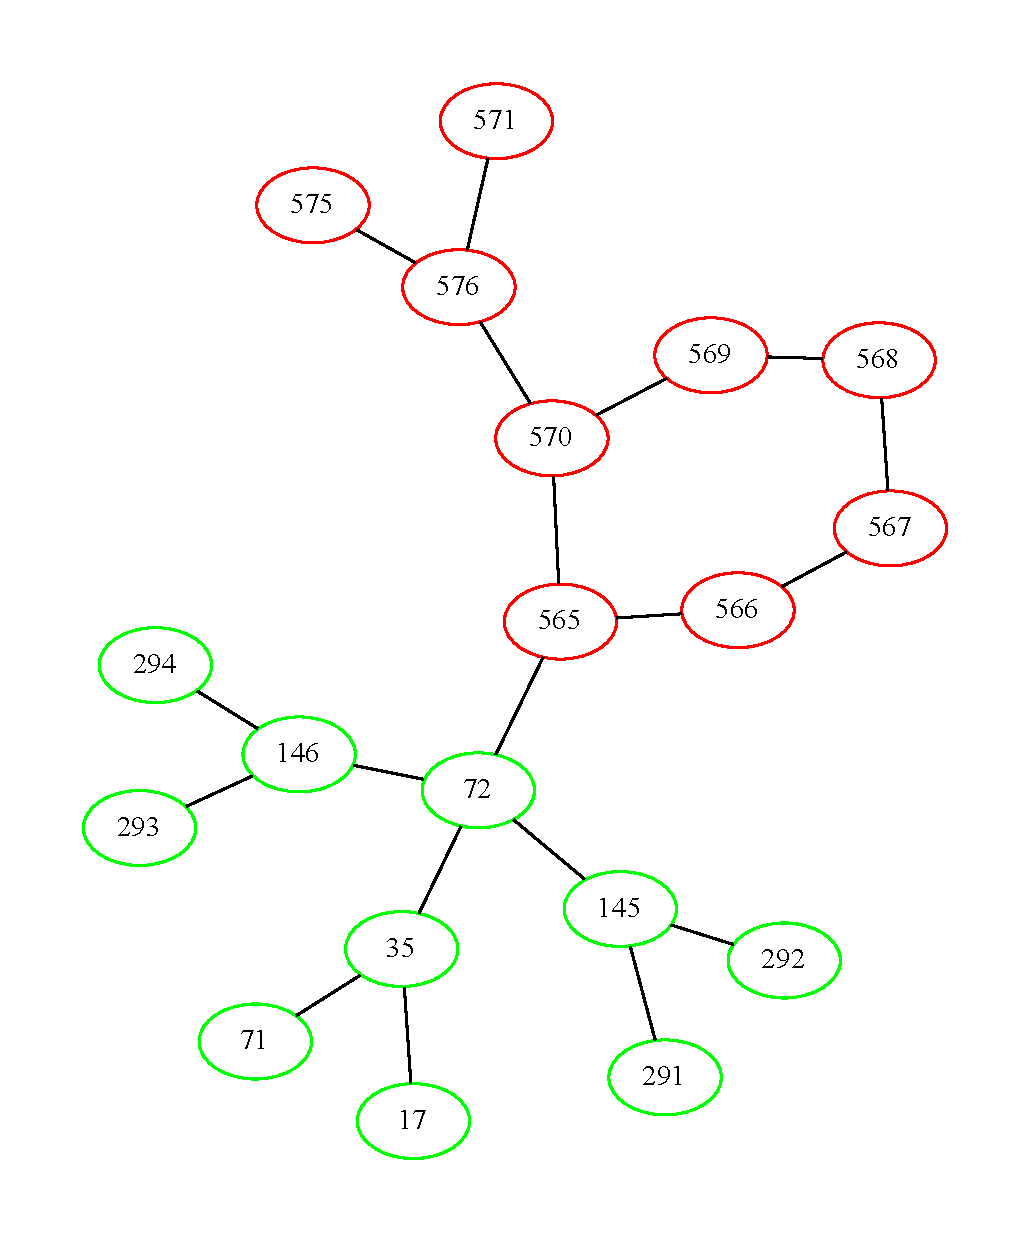
\includegraphics[width=0.6\textwidth]{images/tree-cycles.pdf}
	\caption{A look at the tree-cycles dataset at a three-hop neighborhood around node 565. In green are nodes classified as tree nodes and in red are nodes classified as cycle nodes. The dataset is almost 50\% balanced between these two types.}
	\label{fig:tree-cycles}
\end{figure}

The main dataset focused on in this paper is the Tree-Cycles dataset \cite{ying_gnnexplainer_2019}. In this dataset trees of depth three are attached to cycles of length six in order to form and aggregate dataset. A GNN node classification task entails predicting whether a given node is either in a tree portion of the graph or in the cyclic portion of the graph with no given node features. The idea here is that the GNN can only rely upon the structure of the graph for its node classification and all its information must come from the edges. Hence interpretation on the edges of the GNN would reveal only information that could be gleaned from the graph structure. In figure \ref{fig:tree-cycles}, one can see an example of a portion of the dataset looking at a three-hop neighborhood around node 565.
\begin{figure}[h]
	\centering
	\begin{subfigure}{0.49\textwidth}
		\centering
		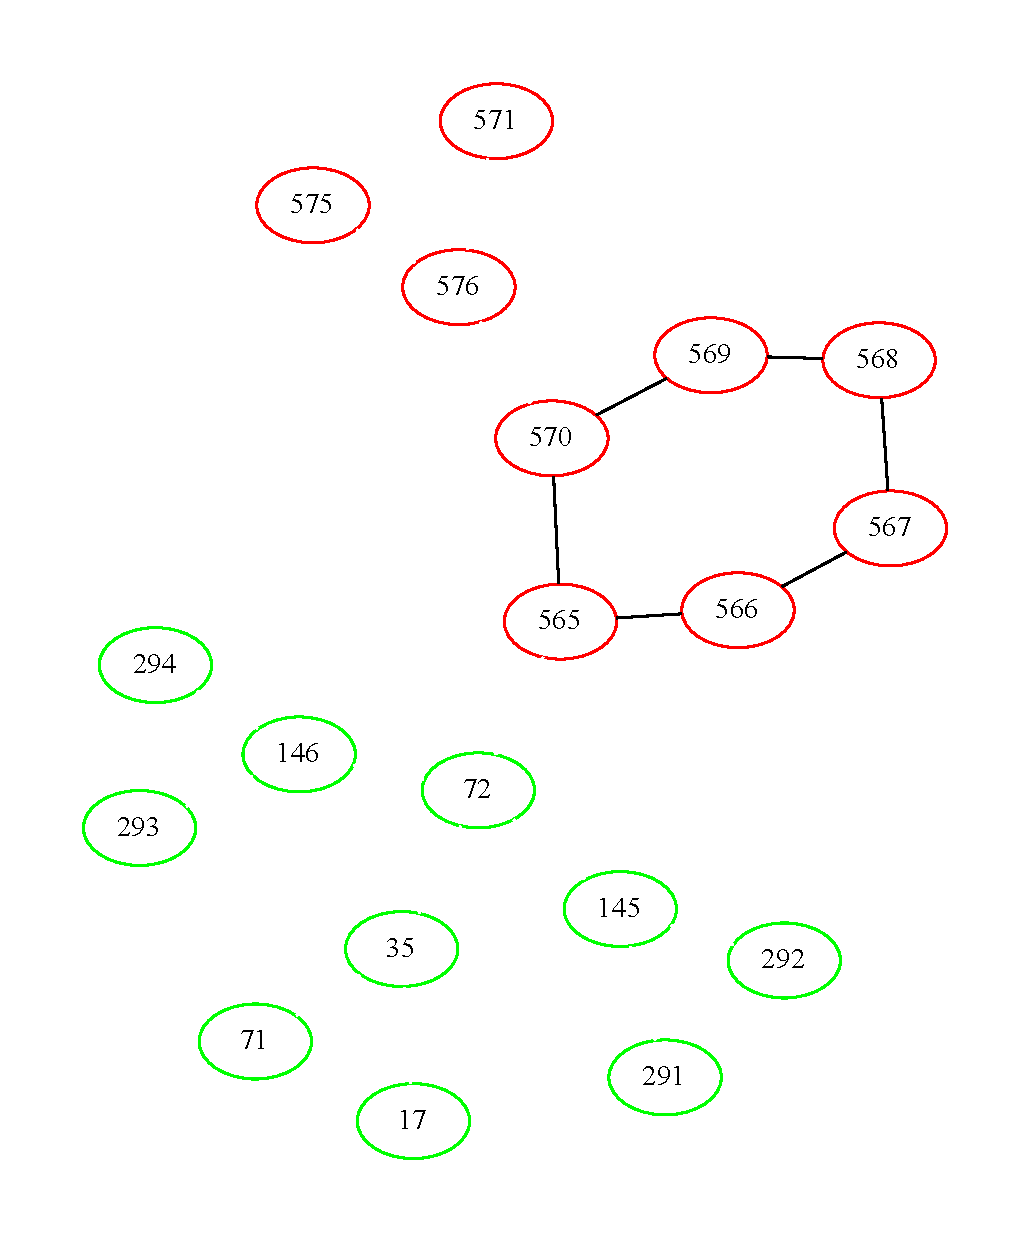
\includegraphics[width=0.9\linewidth]{images/tree-cycles-pos.pdf}
	\end{subfigure}
	\begin{subfigure}{0.49\textwidth}
		\centering
		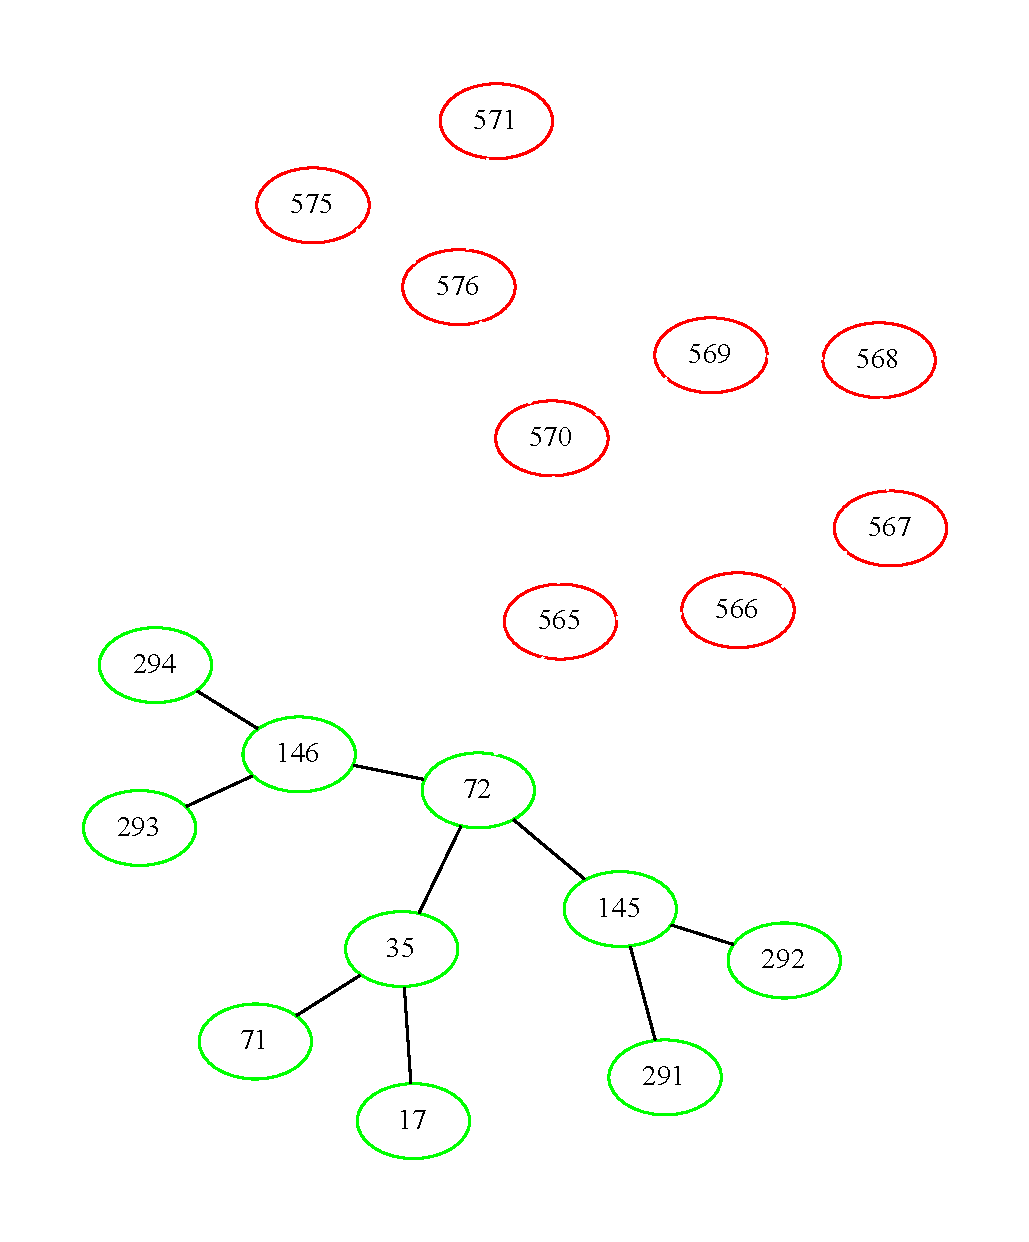
\includegraphics[width=0.9\linewidth]{images/tree-cycles-neg.pdf}
	\end{subfigure}
	\caption{Demonstrations of the proposed groundtruths under \cite{ying_gnnexplainer_2019} for the tree-cycles dataset. On the left is the proposed groundtruth for a node in the cycle (565) and on the right is the proposed ground truth for a node in a tree (72).}
	\label{fig:tree-cycles-proposed-gt}
\end{figure}

While this is a great construction to test an interpretation method, given that the GNN only relies on the graph structure for prediction, it is difficult to imagine what the ground truth for a given dataset is. The paper that introduced GNNExplainer proposed that the groundtruths be motifs in the graph. So if a node was in a cycle portion, the groundtruth would be the edges in the cycle and if a node was in the tree portion, the groundtruth would be the edges of the tree. This can be seen in figure \ref{fig:tree-cycles-proposed-gt} which shows the proposed ground truths. While this is a valid task for an interpretation technique to attempt to solve, it does not have direct bearing on the task that the GNN was trained on and it does not have direct bearing on the mutual information framework that forms the theoretical underpinning for GNN interpretability. 

In a simple example, suppose a GNN is trained on the tree-cycles dataset. While it might be nice if the GNN needed all the edges in a cycle structure to determine that the node is, indeed, in the cycle, the GNN could have just as easily learned to use five edges from the cycle to make its predictions. Even if a theoretical GNN interpretation model was perfect, the fact that the GNN itself does not use the sixth edge means that an interpretation technique is doomed to max its accuracy score at $5/6$ which would make it impossible to compare between methods. Furthermore, a GNN may learn to mix motifs when making its prediction. Consider node 565 in the exampel from figure \ref{fig:tree-cycles}. While this node is in the cycle portion of the graph, the GNN could very easily learn that the node is \textit{adjacent} to the tree structure detected in node 72 and learn to make the inverse decision in this case. Notably, there is no garuntee that a GNN learns the motifs as the important substrucutres and there is little chance that across nodes, it consistently learns these rules. Indeed, it will be shown later that GNNExplainer itself struggles to meet its $>90\%$ accuracy scores for this benchmark in replication studies \cite{yuan_explainability_2021} \cite{lin_generative_2021} and that a thorough search through all connected subgraphs fails to yield this structure as the ground truth. 

While GNNExplainer suggests a few other benchmark datasets, they all suffer from the same issue. Namely, they claim that the groundthruth is the embedded motif structure, but a simple tests reveal that this is not consistently true and nor should it be true in the general case. Hence, a goal of this paper is to also provide a set of alternative benchmarks agaisnt which to evaluate GNN interpretability.

\subsection{Parametrized-Graph Explainer}
Parametrized-Graph Explainer (PGExplainer for short) aims to take the GNNExplainer process and parametrized so that after training a deep neural network, new explanations per node could be generated with the much smaller cost of conducting inference on a give node $v_i$.

In the PGExplainer model, they attempt to construct a generative probablistic model for the underlying subgraph by assuming that the explanatory graph is a Gilbert random graph \cite{gilbert_random_1959} where the edges are conditionally independent of each other, much like GNNExplainer. Hence, the probability of a random subgraph being chosen is given in the same exact way as GNNExplainer. For clarity, this is
\begin{align*}
	\mathcal{P}(\mathcal{W}_i) = \prod_{(v_j, v_k) \in E} \mathcal{W}_i[v_j, v_k]
\end{align*}
and the learning objective, which starts the same as GNNExplainer, becomes the following as they avoid using Jensen's or the mean field approximation
\begin{align*}
	\argmin_{\mathcal{W}_i = q_{\Theta}} \mathbb{E}_{W_i \sim \mathcal{W}_i}[H(\mathcal{P}(\phi(v_i, \mathcal{X}, E, W_i))]
\end{align*}
Note here that the distribution $\mathcal{W}_i$ is to be generated by a DNN that is specified by $q$ and takes as input the parameters $\Theta$. To sample these graphs in a manner that allows for training over the global view of the node classification task, the PGExplainer framework does the following.
\begin{figure}[t]
	\centering
	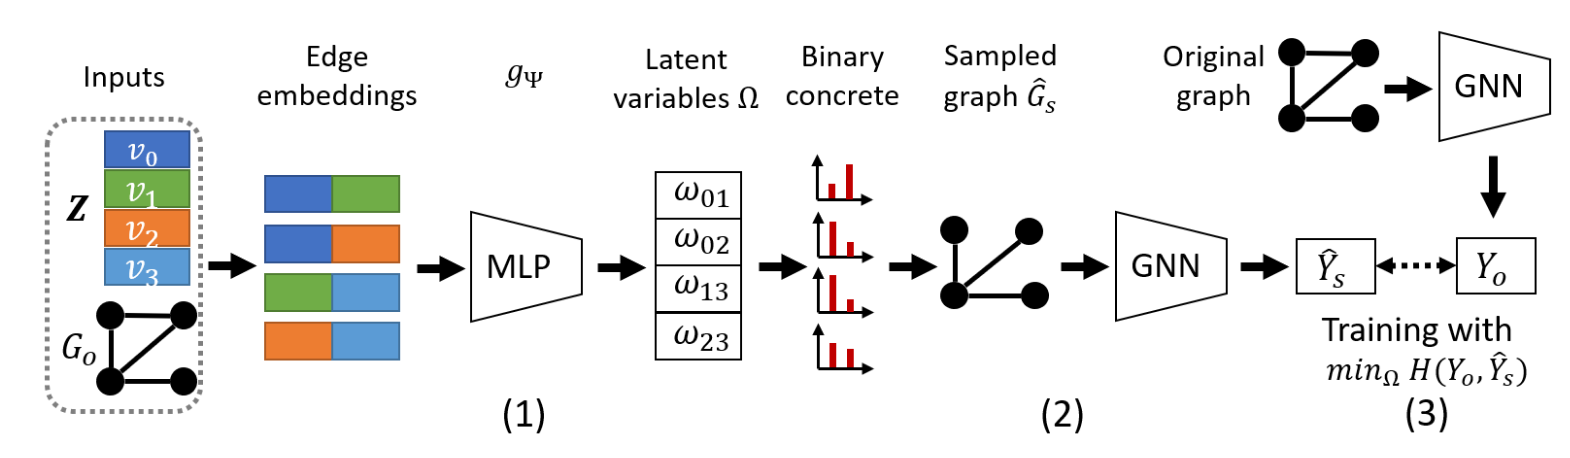
\includegraphics[width=\textwidth]{images/pgexp.png}
	\caption{A convenient overview of the PGExplainer pipeline (with slightly different variable names and setting etc.) \cite{luo_parameterized_2020}}
	\label{fig:pgexp}
\end{figure}
\begin{enumerate}
	\item Most node classification GNNs have a bunch of GNN layers before a final MLP that takes the graph embeddings obtained from the GNN layers and performs a final prediction on the nodes classification. The PGExplainer framework denotes this graph embedding step as $\phi_0$ and extracts it from the GNN task. Let
	\begin{align*}
		Z = \phi_0(v_i, \mathcal{X}, E, W_i)
	\end{align*}
	be the graph embedding calculated with a sampled subgraph $W_i$.
	\item To calculate the distribution $\mathcal{W}_i(v_j, v_k)$, the PGExplainer lets $g$ be a MLP network with shared parameters $\Theta$. As an input, this MLP takes the concatenated values of the graph embedding $Z$ for node $i$ and the nodes $j$ and $k$ as they represent the edge $(v_j, v_k)$. Hence, we have
	\begin{align*}
		\mathcal{W}_i(v_j, v_k) = g_{\Theta}([Z_i; Z_j; Z_k]) \quad\quad \forall (v_j, v_k) \in E
	\end{align*}
	Note here that all edge distributions are independent with respect to $i, j, k$. 
	\item Finally, given this distribution. The parameters $\Theta$ are trained by sampling $K$ subgraphs using the independent edge distributions (utilizing a reparametrization technique) and then optiming the above objective with these samples. Let $W_i^{(k)}$ represent the $k$th sampled subgraph. Then the following objective function represented the final target against which PGExplainer was optimized
	\begin{align*}
		\argmin_{\Theta} -\sum_{v_i \in V} \sum_{k = 1}^K \sum_{c = 1}^C \mathcal{P}(\phi(v_i, \mathcal{X}, E, W) \log \mathcal{P}(\phi(v_i, \mathcal{X}, E, W_i^{(k)}))
	\end{align*}
\end{enumerate}
Together this gives the PGExplainer framework. A convenient outline from their paper can be seen in figure \ref{fig:pgexp}. Note that this framework was tested against the same benchmarks that were given by GNNExplainer. While this gives a more probabilistic framework, it suffers, again, from learning a conditionally independent distribution per edge which disallows further introspection and also ignores the conditional structure while generating subgraphs. This method is better in that it trains these distributions globally across nodes which means that more structure is being captured on the average and allows the model to be universal for a dataset. In effect, the combined training allows for a blurring of the edge importances across different nodes which makes it more useful and generalizable when looking at the edge importance of a specific node.

\subsection{Other Explainer Frameworks}
While there have been a few other explanation frameworks that have emerged in the time following GNNExplainer \cite{ying_gnnexplainer_2019} and PGExplainer \cite{luo_parameterized_2020}, most featured roughly similar performance or design. There are, though a couple frameworks that provide an interesting comparison to the two just mentioned.
\subsubsection{SubgraphX}
This method is different than most methods in that it does not attempt to learn a $\mathcal{W}_i$. Instead, it actively searches for a $\mathcal{E}_i$ and lets $\mathcal{W}_i(v_j, v_k) = 1$ $\forall (v_j, v_k) \in \mathcal{E}_i$. It does this via a Monte-Carlo Tree Search algorithm that is informed by computing Shapley values for proposed subgraph structures and combining them in the tree search \cite{yuan_explainability_2021}. Additionally, this paper eschews the traditional accuracy/AUC evaluation metric used by GNNExplainer and PGExplainer in favor of a Fidelity/Sparsity framework. Crucially, they note that the task being defined by these interpretaion models is not detection of human-interpretable groundtruth motifs, but rather, fidelity to the original predictions made by the full GNN model.
\subsubsection{GEM}
The GEM framework attempts to use Granger Causality to guide its exploration process in learning the $\mathcal{W}_i$ function. The most interesting contribution of this paper to this study was the recognition that the groundtruths determined in the GNNExplainer and PGExplainer works were a bit arbritrary. Certainly, in real-life datasets the motifs that drive a GNN performance are not always apparent and need to be discovered rather than rediscovered. Hence, these benchmarks are a little suspect as they have little bearing on the process of using a GNN interpretation method on a real-world problem.

\subsection{SERGIO}
\label{sec:sergio}
\begin{figure}[h]
	\centering
	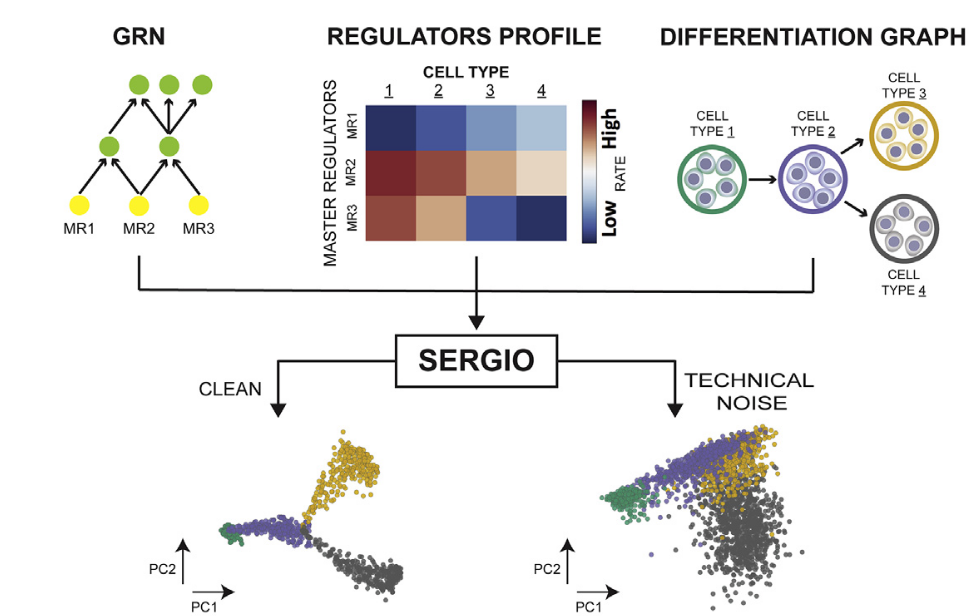
\includegraphics[width=0.8\textwidth]{images/sergio.png}
	\caption{A graphic from the SERGIO paper detailing the inputs and outputs to the SERGIO process \cite{dibaeinia_sergio_2020}. Specifically, a ground truth GRN is utilized to generate the data and recovering this GRN from the data could be a task for a GNN interpretation task.}
	\label{fig:sergio}
\end{figure}
SERGIO is a model for simulating single cell gene expression data with guidance from gene regulatory networks \cite{dibaeinia_sergio_2020}. Before SERGIO, most methods of simulating single cell expression data came from analyzing the statistical properties of real-life single cell datasets and then matching these properties with appropriate distributions that could then be sampled from in order to generate new data. While these methods got more and more sophisticated in the number of statistics they matched against, there was no inclusion of gene regulatory networks (GRNs) which are crucial for single cell expression profiles both in the steady state and dynamical regimesWhile these methods got more and more sophisticated in the number of statistics they matched against, there was no inclusion of gene regulatory networks (GRNs) which are crucial for single cell expression profiles both in the steady state and dynamical regimes.

SERGIO aimed to bridge this gap and created a method that both matched the statistical distributions of experimental expression profiles while utilizing GRNs as the core of the modeling process as seen in figure \ref{fig:sergio}. Crucially, though, the GRN underlying the final expression profile is entirely causal in driving the profiles that it generates and SERGIO maintains the ability to add technical noise into the proposed expression profile. This makes it a perfect setup for an experiment in GNN interpretability where the goal of an interpretation method would be to recover the underlying GRN from a GNN trained on predicting cell type from the expression data. While biological in origin, the abstract problem is perfect for a GNN interpretation task to be benchmarked against.
\newpage
